\documentclass[../../main.tex]{subfiles}
\begin{document}

\begin{flushright}
\footnotesize\textit{【自動文字起こし・要確認】}
\end{flushright}

{\bf [解]}
$C: x^2 + y^2 = 100$ とし, はじめ $C$ と $D$ が $P(10, 0)$ で接しているとする. $D$ の中心を $O_D$ とし, $\angle O_D O A = \theta$ の時の図は右のようになる. この時の $P$ について
\[
\vec{OP} = 7 \begin{pmatrix} \cos\theta \\ \sin\theta \end{pmatrix} + 3 \begin{pmatrix} \cos(-\dfrac{7}{3}\theta) \\ \sin(-\dfrac{7}{3}\theta) \end{pmatrix} = \begin{pmatrix} x(\theta) \\ y(\theta) \end{pmatrix}
\]
が成り立つ.
\begin{align}
\circ \ x'(\theta) &= -7\sin\theta - 7\sin\dfrac{7}{3}\theta = -7 \cdot 2 \sin\dfrac{5}{3}\theta \cos\dfrac{2}{3}\theta \\
\circ \ y'(\theta) &= 7\cos\theta - 7\cos\dfrac{7}{3}\theta = 7 \cdot 2 \sin\dfrac{5}{3}\theta \sin\dfrac{2}{3}\theta
\end{align}
から下表をうる.

\begin{center}
\begin{tabular}{|c|ccc|}
\hline
$\theta$ & $0$ & $\dots$ & $\dfrac{3}{5}\pi$ \\ \hline
$x'$ & $0$ & $-$ & $0$ \\ \hline
$y'$ & $0$ & $+$ & $0$ \\ \hline
$(x, y)$ & $(10, 0)$ & & \\ \hline
\end{tabular}
\end{center}

したがって, $P$ の軌跡の概形は右図, 斜線部の面積を $T$ とすると
\begin{align}
T &= \int_{10\cos\frac{3}{5}\pi}^{10} y \, dx = \int_{\frac{3}{5}\pi}^0 y \dfrac{dx}{d\theta} \, d\theta \\
&= \int_{\frac{3}{5}\pi}^0 \left( 7\sin\theta - 3\sin\dfrac{7}{3}\theta \right) \left\{ -7\sin\theta - 7\sin\dfrac{7}{3}\theta \right\} d\theta \\
&= 7 \int_0^{\frac{3}{5}\pi} \left( 7\sin^2\theta - 3\sin^2\dfrac{7}{3}\theta + 4\sin\theta\sin\dfrac{7}{3}\theta \right) d\theta \quad \cdots ①
\end{align}

各項計算して
\[
\int_0^{\frac{3}{5}\pi} \sin^2\theta \, d\theta = \dfrac{1}{2} \left[ \theta - \dfrac{1}{2}\sin 2\theta \right]_0^{\frac{3}{5}\pi} = \dfrac{1}{2} \left( \dfrac{3}{5}\pi - \dfrac{1}{2}\sin\dfrac{6}{5}\pi \right)
\]
\[
\int_0^{\frac{3}{5}\pi} \sin^2\dfrac{7}{3}\theta \, d\theta = \dfrac{1}{2} \left[ \theta - \dfrac{3}{14}\sin\dfrac{14}{3}\theta \right]_0^{\frac{3}{5}\pi} = \dfrac{1}{2} \left( \dfrac{3}{5}\pi - \dfrac{3}{14}\sin\dfrac{14}{5}\pi \right)
\]
\begin{align}
\int_0^{\frac{3}{5}\pi} \sin\theta\sin\dfrac{7}{3}\theta \, d\theta &= \int_0^{\frac{3}{5}\pi} -\dfrac{1}{2} \left( \cos\dfrac{10}{3}\theta - \cos\dfrac{4}{3}\theta \right) d\theta \\
&= -\dfrac{1}{2} \left[ \dfrac{3}{10}\sin\dfrac{10}{3}\theta - \dfrac{3}{4}\sin\dfrac{4}{3}\theta \right]_0^{\frac{3}{5}\pi} = +\dfrac{3}{8}\sin\dfrac{4}{5}\pi
\end{align}

①に代入して
\begin{align}
T &= 7 \left[ 7 \left( \dfrac{3}{10}\pi - \dfrac{1}{4}\sin\dfrac{6}{5}\pi \right) - 3 \left( \dfrac{3}{10}\pi - \dfrac{3}{28}\sin\dfrac{14}{5}\pi \right) + 4 \cdot \dfrac{3}{8}\sin\dfrac{4}{5}\pi \right] \\
&= 7 \left[ \dfrac{6}{5}\pi + \dfrac{25}{14}\sin\dfrac{1}{5}\pi \right]
\end{align}
だから, 小さい方の面積 $S_1$, 大きい方のそれを $S_2$ として,
\begin{align}
S_1 &= \text{[扇形]} - T \\
&= 30\pi + \dfrac{1}{2} \cdot 100 \sin\dfrac{2}{5}\pi \cdot \cos\dfrac{2}{5}\pi - \dfrac{42}{5}\pi - 25\sin\dfrac{1}{5}\pi \\
&= \dfrac{108}{5}\pi
\end{align}
\[
S_2 = 100\pi - S_1 = \dfrac{392}{5}\pi \quad \text{//}
\]

\begin{center}
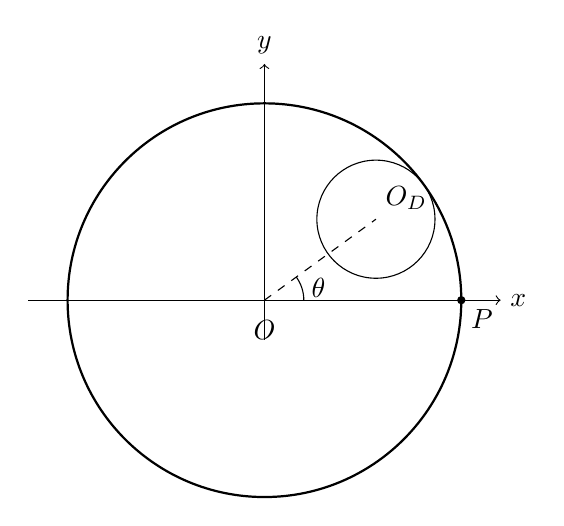
\begin{tikzpicture}[scale=0.25]
  \draw[->] (-12,0) -- (12,0) node[right] {$x$};
  \draw[->] (0,-2) -- (0,12) node[above] {$y$};
  \draw[thick] (0,0) circle (10);
  \coordinate (O) at (0,0);
  \coordinate (Od) at ({7*cos(36)},{7*sin(36)});
  \draw[dashed] (O) -- (10,0);
  \draw[dashed] (O) -- (Od);
  \draw (Od) circle (3);
  \fill (10,0) circle (6pt) node[below right] {$P$};
  \node at (0,-1.5) {$O$};
  \node at (Od) [above right] {$O_D$};
  \draw (2,0) arc (0:36:2) node[midway,right] {$\theta$};
\end{tikzpicture}
\end{center}

\end{document}
